\begin{figure}[htbp]
\centering
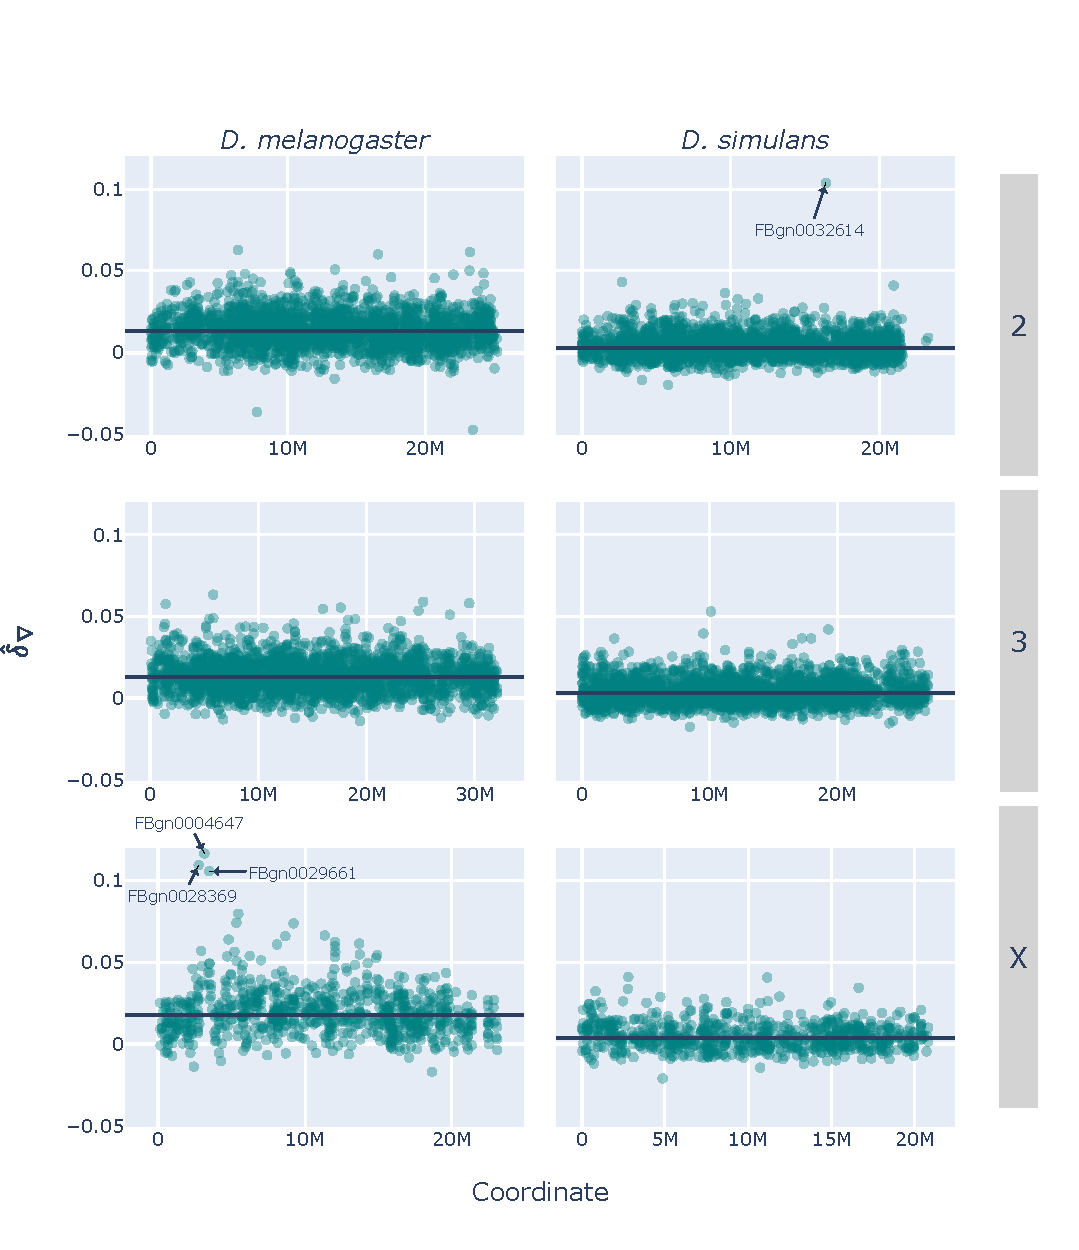
\includegraphics[width=\textwidth]{figures/plots/drosophila/d-conv_manhatten.pdf}
\caption[The pattern of elevated mutation disequilibrium in \textit{D. melanogaster} compared to \textit{D. simulans} is systematic across the genome]{\textbf{The pattern of elevated mutation disequilibrium in \textit{D. melanogaster} compared to \textit{D. simulans} is systematic across the genome}. Manhattan plots the position of a gene in a chromosome and the $\hat\delta_\nabla$ for the CDS sequence of that gene. The CDS sequence is third codon position only. The median $\hat\delta_\nabla$ is indicated for a chromosome with a horizontal line. The number of genes included in the plots of chromosome 2, 3, and X of \textit{D. melanogaster} is 2,373, 2,624 and 818 respectively. For chromosome 2, 3, and X of \textit{D. simulans}, the number of genes is 2,388, 2,623 and 800 respectively.}
\label{fig:drosophila_d-conv_manhattan}
\end{figure}
